\chapter{Progress, Timeline, and Outlets} \label{ch:[chapter 7 label]}

The progress of this research will be evaluated monthly. Based on the research design, a study will commence once the previous one has been completed. However, at this point, I have made some progress on most of the studies. The majority of my progress concerns studies one and two. In study one, I have surveyed five portals and recorded their search facets. I have found that all of them allow users to input keyword searches and most of them allow further query specifications by filtering results based on tags, and formats. Most portals allow ordering results by "relevance", creation date, and alphabetically. I have found that at least three portal search systems are built on Apache Lucene and at least two on CKAN. I have begun executing predetermined queries, and recording results and how they change.

In study two, I have spent most of the time pre-processing the query logs. I am almost finished constructing a parsing pipeline that includes topic modelling, dependency parsing, and geoparsing. I have calculated descriptive statistics of query terms including descriptions of word and phrase frequencies and topic distributions among others. In study four, I have deconstructed the existing scoring/ranking function used in OpenData and tested simple system modifications such as changing word weighting from a TF-IDF to Okapi BM25.



Figure \ref{fig:Timeline} depicts my timeline for completing this research as well as likely outlets for each study. I accept that this timeline will possibly change, but I remain determined to complete my studies by the end of the 2021 academic year. I recognize several situations that may delay or prolong a study. For example, study two may require that I manually construct a test collection in order to be useful for studies four and five. Furthermore, I may not be able to set up a mature A/B user test environment since this takes significant resources. However, since I am in close collaboration with Esri and may be hired by them to continue this work, creating some sort of user testing environment shouldn't be a problem.

\begin{figure}[H]
    \centering
    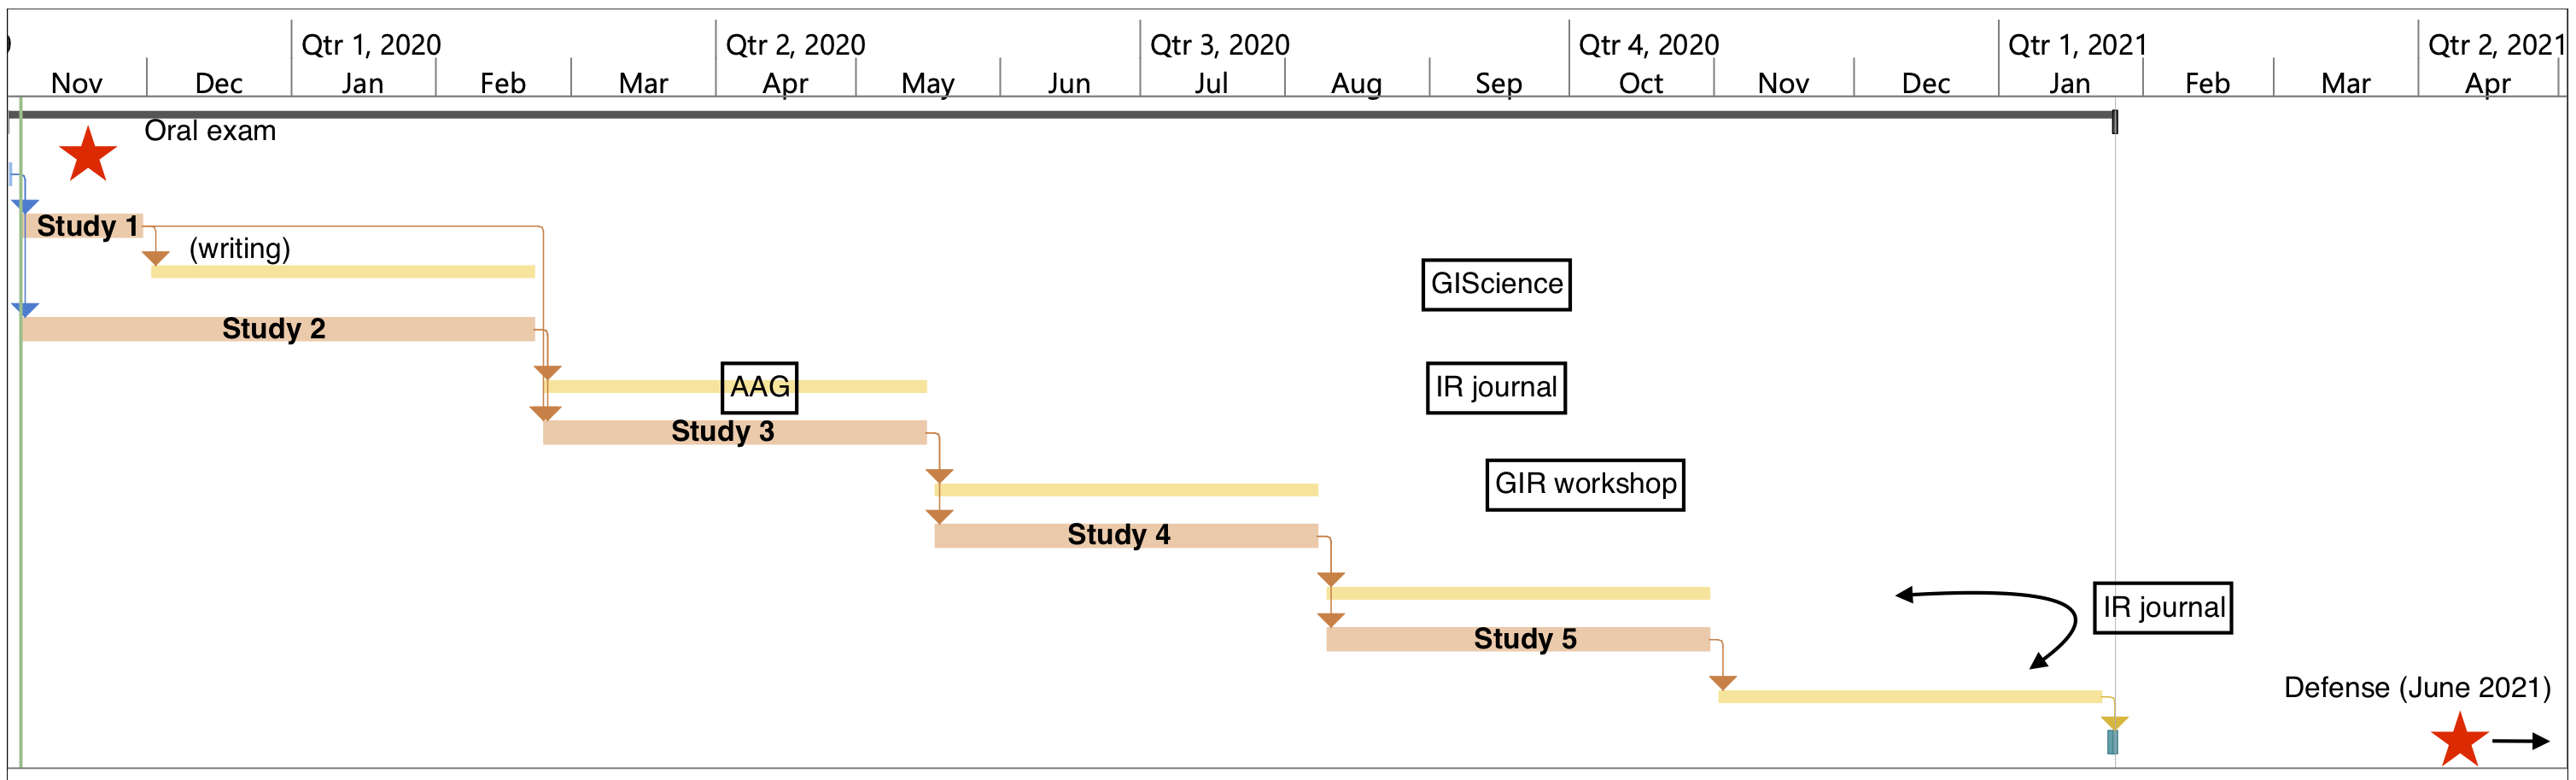
\includegraphics[width=1\textwidth]{../figures/Timeline.png}
    \caption{Research timeline by study. Each study has a work phase (orange) and a subsequent writing phase (yellow). Outlets for the studies are highlighted during or after the writing phase including the GIScience and AAG conferences, IR journals, and the annual GIR workshop.}
    \label{fig:Timeline}
\end{figure}